\chapter{Proposed Algorithm}

This section deals with the application of BCD search for the converging to the solution. There are numerous methods available for finding the global optimum. \cite{Forrester2008}
Meta-heuristic methods like genetic algorithm, simulated annealing are gaining popularity, however, their convergence rate is very slow. Deterministic methods like Branch-and-Fit use Lipschitzian-based partitioning techniques but the problem of finding the Lipschitz constant is sometimes as hard as solving the problem itself. \cite{Strongin1973}  Although there are methods to approximate the Lipschitz constant, a big disadvantage of Lipschitz optimization methods is the need for plenty of function evaluations to get a good estimate of the optimal point. 
On the other hand, using surrogate models is increasing in popularity as the surrogate modeling capabilities for the objective and constraint functions that can be used for optimization have immensely improved. Moreover, computational time is saved by parallelizing the runs used to fit the surfaces. \cite{Jones2001}
Another advantage of the approach is that statistical analyses and experimental design can be done to identify which input variables are the most important by finding the variable contributing the highest variance to the output.

% Pseudo code
\begin{algorithm}
   
\end{algorithm}

% Sampling methods
\section{Sampling methods}
With function evaluations being computationally expensive, it is essential for the algorithm to select adaptively the points to evaluate over for building the surrogate model. During initial investigation of the modeling, it was observed that the surrogate model built by low-discrepancy sequences or the quasi-random sequences was able to generalize to the model much better than the points sampled randomly. 
The quasi-random sequences are able to cover larger domain space with the same number of evaluation points since the points sampled are not completely independent of the previously sampled points. The sampling techniques used are discussed below.

% Latin hypercube sampling
\subsection{Latin hypercube sampling}
Widely used in the Monte Carlo simulation, Latin hypercube sampling divides the search domain into N intervals of equal probability. This sampling then selects one sample from each of these intervals. 

\subsection{Sobol sampling}

In 1967, Ilya Sobol introduced the Sobol sequencing, which tries to sub-divide the M-dimensional space into $2^M$ points. We get data points $x$ as:

\begin{center}
$x \in \Big \{\displaystyle \frac{k}{2^M}, k \in [0,1,..2^M-1] \Big \}$
\end{center}

\noindent
In order to have each of the points to have low discrepancy, some Generative matrices are selected which would mimic the points sampled in a dimension. For instance, for M = 2 dimensions and N = 4, we can have
% \usepackage{amsmath}
\begin{singlespace}
\[C_{x} = 
\begin{pmatrix}
    1 & 0 & 0 & 0       \\
    1 & 1 & 0 & 0       \\
    1 & 0 & 1 & 0       \\
    1 & 1 & 1 & 1       \\
    
\end{pmatrix}
, 
\begin{pmatrix}
    1 & 0 & 0 & 0       \\
    0 & 1 & 0 & 0       \\
    0 & 0 & 1 & 0       \\
    0 & 0 & 0 & 1       \\
      
\end{pmatrix}
, etc.
\]
\end{singlespace}
\bigskip
\noindent
Using these generative matrices, points for each of the dimensions are selected as:
\begin{center}
$x_{n} = \displaystyle \sum_{M-1}^{k=0} t_{k}2^{-k-1}$
\end{center}

\bigskip
\noindent
where $t = \sum_{i}2^{i}m_{i}$. An important property of Sobol sampling is that if there are more points than $2^N$, then the $x_n$ computed for the additional points would occupy the finer spaces of each axes. 	

%Hammersley sampling
\subsection{Hammersley sampling}
Hammersley sampling was introduced in 1975, which is an adaptation of the Halton sequence. We select a set of primes $p_{j}, j \in (1,.. N-1)$
For a given prime (p), if the van der Corput sequence is given by $g_{p}(n)$, then while the $i^{th}$ sample point for Halton is $x_{i} = (g_{p_{1}}(i), g_{p_{2}}(i), .., g_{p_{n}}(i) )$, for Hammersley, the $i^{th}$ sample point is $x_{i} = (i/N, g_{p_{1}}(i), g_{p_{2}}(i), .., g_{p_{n-1}}(i) )$
The Halton and Hammersley sampling is simple and efficient and both achieve asymptotically optimal discrepancy.

% Latex
% \usepackage{subcaption}

\begin{figure}
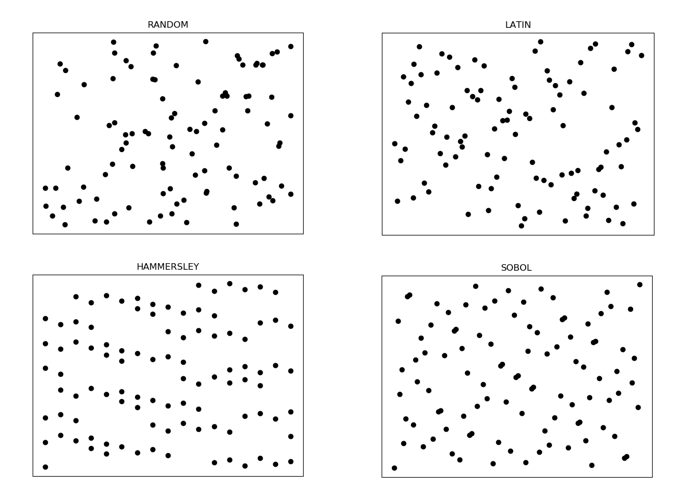
\includegraphics[width=0.9\textwidth]{all_sampling_methods.PNG}
\caption{Sampling for 100 points carried out by (a) Random, (b)  Latin Hypercube, (c) Hammersley, and (d) Sobol sampling in 2 dimensions.}
\label{fig:Sampling}
\end{figure}

\bigskip
\noindent
All the sampling methods are can be collectively compared as in Figure \ref{fig:Sampling}. In general, quasi-random sampling techniques are able to sample points from a larger area for the same number of evaluations. For test problems, it was observed that convergence of the model required about half the number of function calls compared to random sampling. Since Sobol sequences can converge faster than other simpler sampling techniques, for all the calculations in the report, Sobol sampling was used unless other method was mentioned.

% Alamo
\section{Surrogate model function}
After sampling the points, a surrogate function is fit on the points. There are plenty of options to build the model. The basis of selecting the right modeling technique is that the function must neither be too simple that it might require several iterations nor be too complex to generalize and be unable to provide the right point for next iteration.
\bigskip
\noindent
To develop good approximation models, response surface methodology will be designed for the system being analyzed. In response surface methodology, scattered data is modeled assuming it will possesses some local/global optima. In general, we assume that we are analyzing the following complex system:
\begin{center}
$y=F(x)$,
where $x=[x_{1}, x_{2}, .., x_{m}]^{T}$    
\end{center}
\noindent
For analysis, we have N sampled points $x_{i}$ with corresponding output values $y_{i}$, i = 1,2,…, N. While optimizing using linear or quadratic least square approach provides useful information about the model, it fails to locate multiple minimas or maximas. For this reason, the modeling carried out is not on very simple algebraic functions. Three methods used in this work are discussed below.

\subsection{Radial Basis Function}
The Radial Basis Functions (RBF) uses a function $\phi(\cdot)$, whose value at any given point (x) depends upon distance from the known sampled points. The $\phi(\cdot)$ depends on the kernel selected and for the investigations in this work is set to a polynomial of third order [1]. The function value F(x) is found as:  

\begin{center}
    $F(x) = \displaystyle \sum_{M-1}^{k=0} w_i\phi(r_i, c)$
\end{center}

where $w_i$ is coefficient for $i^{th}$ point $r_i$ is the distance of point x from the $i^{th}$ sampled point. The linear model formation of F(x) allows the estimation of the optimal parameter value $w_i$ using linear least squares. The RBF algorithm \ref{alg:rbf} is inspired from \cite{Mller2013}.


% MULTILINE INDENTATION 
% \State \multiline{%
%             Get $f_{min}$ and $f_{max}$ to set $f_p(z_i) \forall i$
%             \Comment{$f_p(z)$ is $f(z)$ with penalty term}}

\begin{algorithm}
\caption{RBF algorithm}\label{alg:rbf}
\begin{algorithmic}[1]
\Procedure{RBF modeling}{$a,b$}
\State Set $C \gets 0$   
\Comment{Initialize the evaluation count}
and s to get 
\State Sample $z_i, f(z_i)$ and get $z_{min}$

\While{$C<$ Max function evaluations}
\State Get $f_{min}$ and $f_{max}$ to set $f_p(z_i) \forall i$
            \Comment{$f_p(z)$ is $f(z)$ with penalty term}
\State Create an rbf model $p(z)$ over these points
\State $V_R(x_j) = \displaystyle\frac{s_p(x_j)-s_{min}}{s_{max}-s_{min}}$
\Comment{$s_p(z_i)=\sum\lambda_i\phi+p(z)$}

\State $V_D(x_j) = \displaystyle\frac{\Delta_{max}-\Delta(x_j)}{\Delta_{max}-\Delta_{min}}$
\Comment{$\Delta(x)$ is the distance of $x_j$ from closest $z_i$}

\Statex Get the scoring using both $V_R$ and $V_D$. Their weights are cyclically updated as: Initialize $W_R=0$ and $W_D=1$, iteratively decrease $W_D$ to 0 and reset it to initial values.
\State W($x_j$) = $W_RV_R(x_j) + W_DV_D(x_j) $
\State Select the candidate point with best score, 
\State Sample around it to get $z_i, f(z_i)$ and $z_{min}$

\EndWhile\label{RBFendwhile}
\State \textbf{return} $z_{min}$
\EndProcedure
\end{algorithmic}
\end{algorithm}

This algorithm had to be used since the scoring criteria based on distance parameter $V_D$ has to be used only in an RBF model.

\subsection{Multi-layer Perceptron}
In the past few years, neural network based models have become a useful tool for regression problems. A Multi-layer Perceptron (MLP) is called a universal function approximator as it can fit on any given input-output data pair. The main challenge with respect to applying this in black-box problem is in deciding the model architecture. The algorithm must be able to handle any new black-box function with any number of input features. In addition, the underlying model can have varying complexity. Moreover, the objective of the surrogate model building is to build a generalized model using the least number of sample points. Thus, building a custom architecture for each model is not feasible and hence we must build a model for each iteration of BCD with the limited number of samples.
\bigskip
\noindent
Using Tensorflow, an MLP was designed with single hidden layer on which an activation function of Rectified Linear Unit (ReLU) was applied. Since fitting this model to highly complex function might cause large error, the LOGCOSH was chosen as the loss function. Considering $x$ as the error, if $x$ is small, $log(cosh(x))$ is approximately equal to $x^2 / 2$ and if $x$ is large then it is $abs(x) - log(2)$. This loss function was selected rather than mean squared error in order to avoid very high loss values that may cause high variation in training. The training of the function was carried out using ADAM optimizer owing to its ability to handle sparse gradients on noisy problems (8). To converge to a new point, the MLP iterates as 
\begin{center}
$X_{i+1} = X_i - \nabla (X_i)*\lambda$
\end{center}
For optimization, only four iterations were used in each instance to reach a sub-optimal solution. For this reason, the learning rate was kept higher ($\lambda = 0.25$) than usual of to reach the gradient solution quicker.

\subsection{ALAMO (Automated Learning of Algebraic Models for Optimization)}

The last method used for modeling is ALAMO, which is a modeling toolbox built specifically for black-box problems. The main challenge solved by ALAMO \cite{Lindqvist2018} is in determining simulation domain by carrying out adaptive sampling and fitting low complexity surrogate models.
In order to obtain such low complexity models, ALAMO allows various basis functions as observed in Table below (make table of various options).
Various combinations of simple basis functions are considered for generating algebraic models, which are then solved using an optimization framework. 

\bigskip
\noindent
The sampling ALAMO uses is an active learning approach for selecting the next set of points that can achieve best accuracy using minimum evaluated points. An error-maximization strategy is employed to ensure that the points having the largest deviation from the model are included in model building for subsequent iterations. 

\bigskip
\noindent
In order to obtain such low complexity models, ALAMO allows various basis functions that we would want the function to be modeled on. ALAMO can model functions with polynomial, logarithmic, exponential and trigonometric terms. Since this work iterates while converging to the solution and only a small set of points are used keeping the function evaluation budget in mind, the options were set to model a second order polynomial function. 

\bigskip
\noindent
The sampling ALAMO uses is an active learning approach for selecting the next set of points that can achieve best accuracy using minimum evaluated points. An error-maximization strategy is employed to ensure that the points having the largest deviation from the model are included in model building for subsequent iterations. 

\subsection{Selection of modeling method}
In order to design the hyperparameters for the modeling algorithm, selection of one of the three methods discussed is vital. The modeling with the MLPs with variation in various hyperparameters was not able to provide good results since it cannot model with the limited number of evaluation points provided. When comparing the results found by modeling with the radial basis function and ALAMO, it was found that the former model's convergence stopped when the dimensions of the black-box function was more than 50. Hence, for rest of the work, the modeling was carried out using ALAMO.

% Optimizers
\section{Optimizers}
The functions returned by ALAMO are such that they are linear combinations of differentiable functions (like trigonometric, exponential, or polynomial). The algorithm is designed such that the optimizer selected needed to solve bounded minimization problems. Since we are fitting polynomial models, the following optimizers can be used.

\subsection{L-BFGS-B method}
The BFGS method is a quasi-Newton method (methods not requiring Hessians), so the Hessian matrix is approximated by evaluating gradients. The BFGS has better performance compared to Newton’s method for non-smooth optimization instances. In order to accommodate for bounded constraints, BFGS-B variant of the algorithm is used. In order to optimize for large number of variables, the limited memory version of it called the L-BFGS-B (Limited-memory BFGS bound-constrained) method is used. 

\subsection{SLSQP method}
The SLSQP (Sequential Least Squares Quadratic Programming) is also a quasi-Newton method and it iterates in a Sequential Quadratic Programming (SQP) manner, In order to enforce constraints, the first and second order optimality conditions are applied.

\subsection{TNC method}
The TNC (Truncated Newton Constrained) algorithm uses gradients \cite{Nash1984} like the Newton-Conjugate gradient method and not the Hessian matrix. It also allows each variable to be given upper and lower bounds.  
Being truncated, the inner solver has limited number of iterations. Thus, this optimizer requires that the inner algorithm has low condition number for the Preconditioned iterative method.

\bigskip
\noindent
For the given problem set, all of the solvers perform equally well in helping the algorithm converge to the solution. However, since the variable size can be varying, L-BFGS-B is chosen  as it is tweaked to work efficiently when there are large  number of variables to be optimized.

% Implementation of CCS 
\section{Cyclic Coordinate Search}

This section describes the methodology of how the algorithm works. For this algorithm, the sampling technique, number of starting points, and tolerance of improvement can be provided or the default values are taken. Since the optimization is carried out in a block coordinate manner, the number of features (m) and the points (N) to be sampled have to be specified.  

\begin{algorithm}
% \caption{RBF algorithm}\label{alg:rbf}

% \State \multiline{% 
%             Get sample points in m dimensions
%             \Comment{If }}
\begin{algorithmic}[1]
\Procedure{New point}{oldData, p}
% \Comment{The g.c.d. of a and b}
\State \multiline{% 
Presently at $X_0,Y_0$, the points are sampled about m attributes of $X_0$
\Comment{This function iterates until improved point is found or the patience factor is 0}
}

\If {oldData is None} 
    \State Sample N points of $(x^{(m)}, y)$
\Else       
    \State Sample N more points of $(x^{(m)}, y)$ and merge this with the oldData
\EndIf

\State Build a model $f^{A}(\cdot)$ using ALAMO 
\State \multiline{% 
Minimize $f^{A}(\cdot)$ to predict new $x^*$ and get $y^*=f(x^*)$
\Comment{$f(\cdot)$ is the black-box function evaluation}
}
\If {$p>0$}  \Comment{The patience factor (p) of recursion at this point}
    \State Sample N points of $(x^{(m)}, y)$
    \If {$y_{min}<Y_0$ }  \Comment{$y_{min} = min(y^*, y_i) \forall i$}
        \State $Y_0 \gets y_{min}$
        \State $X_0 \gets x_{min}$  \Comment{$y_{min} = f(x_{min})$}
        \State Apply scaling factor across these m features
    \Else
        \State $p \gets p-1$
        \State Add new points to oldData and call the NEW POINT(oldData, p) function
    \EndIf
    
\Else
    \State Return with same point and iterate over other attributes
\EndIf

\State \textbf{return} $X_0, Y_0$   
\Comment{Updated optimal point across m attributes}
\EndProcedure
\end{algorithmic}
\end{algorithm}

\noindent
The main algorithm uses the above procedure for optimizing along the selected coordinates. The work is inspired from the Boosting with Momentum concept utilized in \cite{Mukherjee2013}. In the coordinate search, each coordinate step is termed as an iteration and an iteration over all the variables is called an epoch. Following each epoch, the momentum in that epoch is added to boost the convergence. Additionally, the variables are sorted using the momentum values in order to make surrogate functions more representative, else the surrogate model built only has variables with higher momentum.

\bigskip
\noindent
Various starting points are sampled to start iterating if the improvement in previous epoch was not significant, indicating a local or global minima point. In this work, a relative improvement of minimum $0.1\%$ was needed; else the algorithm iterates over next starting point.

\begin{algorithm}
\caption{Main algorithm}\label{alg:rbf}
\begin{algorithmic}[1]
\Procedure{Boosting with Momentum}{}
% \Comment{The g.c.d. of a and b}
\State Set $C \gets 0$   \Comment{Initialize the evaluation count}

\State Sample multiple starting points $(X^{SP}_k, Y^{SP}_k)$ and sort based on output.

\While{$C<$ Max function evaluations}

  \While{$E<$ MaxEpochs}
  \State Start this epoch from $(X^{E},Y^{E})$
  \State Set axis order using $\Delta X^{E-1}$ for epoch E
    \For{$i\in[1,B]$}  \Comment{B is number of blocks}
    
    \State Add momentum along the axes selected in $i^{th}$ iteration
    
    \State $X_i^{E} \gets X_i^{E} + \beta(\Delta X_i^{E-1})$
    \State $Y_i^{E} \gets f(X_i^{E})$
    
    \State Optimize across this point using Surrogate model
    
    \State $X_i^{E}, Y_i^{E} \gets$ NEW POINT$([X_i^{E}, Y_i^{E}],0)$
   
    \EndFor
    
    \State Compute the momentum in this epoch
    \State $\Delta X^{E} \gets X^{E} - X^{E-1}$
    \State $\Delta Y^{E} \gets Y^{E} - Y^{E-1}$

    \If {$\Delta Y^{E} < j$}  \Comment{Significant decrease in Y value}
    
        \State Continue to next epoch
        
    \Else           \Comment{Point has not improved significantly}
        \State Start from next best starting point
    \EndIf
    
  \EndWhile\label{MaxEpochs} 
  \Comment{Start iterating from next starting point}

\EndWhile\label{FunctionCalls}


\EndProcedure
\end{algorithmic}
\end{algorithm}

